% Preamble
% Compile with XeLateX

\documentclass[11 pt,oneside,a4paper,titlepage]{article}
\usepackage{preamble}
\graphicspath{{PIC/}}
%%%%%%%%%%%%%%%%%%%%%%%%%%%%%%%%%%%%%%%%%%%%%%%%%%%%%%%%%%%%%%%%%%%%%%%%%%%%%%%%%%%%%%
\begin{document}

\sidebar{sideBarColor!25}
\simpleheader{titleBackColor}{Frederik}{Laubisch}{Data Engineer | Cloud Engineer}{white}

% Start Minipages
\vspace*{3.49cm}% start 8 cm from the top of the page}
    \adjustbox{valign=t}{\begin{minipage}[t]{6.4cm} % large 7.4 cm from the top
    \vspace*{1.6cm} % text starts 1cm under the top of the minipage

        % Picture
        \begin{center}
        \begin{tikzpicture}
            \node[
            circle,
            minimum size=\cvPictureWidth,
            path picture={
            \node at (path picture bounding box.center){
             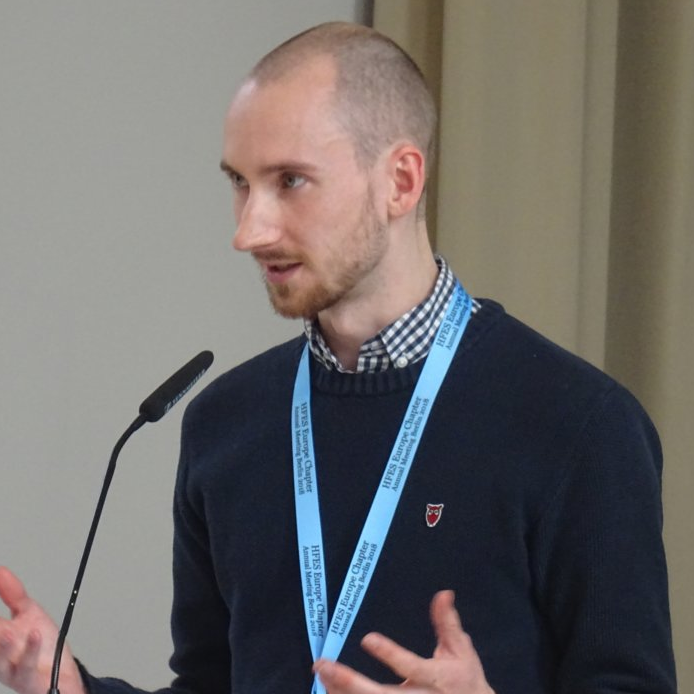
\includegraphics[width=\cvPictureWidth]{FreddySquared.png}
             };
             }]
            {};
        \end{tikzpicture}
        \end{center}

        %%%%%%%%%%%%%%%%%%%%%%%%%%%%%%%%%%%%%%%%%%%%%%%%%%%%
        % Profile section
        \ruleline{\textbf{Über mich}}
        Ursprünglich in Kognitionswissenschaft und Human-Factors-Forschung ausgebildet, wechselte ich in die Daten- und Cloud-Entwicklung \textemdash{} angetrieben von der Leidenschaft, Technologien mit echtem Praxisnutzen zu entwickeln.
        \vspace*{0.8cm} % text starts 0.4cm under the top the header

        %%%%%%%%%%%%%%%%%%%%%%%%%%%%%%%%%%%%%%%%%%%%%%%%%%%
        % Contact Section
        \ruleline{\textbf{Kontakt}}
        \begin{tikzpicture}[every node/.style={inner sep=0pt, outer sep=0pt}]
        \matrix [
        column 1/.style={anchor=center,contactIcon},
        column 2/.style={anchor=west,align=left,contactIcon},
        column sep=5pt,
        row sep=5pt] (contact) {
        \node{\faMale};
         & \node{Geboren am 29.01.1990};\\
        \node{\faEnvelope};
         & \node{\protect\href{mailto: f.laubisch@posteo.de}{f.laubisch@posteo.de}};\\
        \node{\faPhone};
         & \node{+49 157 78944004};\\
        \node{\faMapMarker};
        & \node{Merianstr. 32A \\ 79104 Freiburg im Breisgau \\ Deutschland};\\
        \node{\faLinkedinSquare};
        & \node{\href{https://www.linkedin.com/in/frederik-laubisch/}{frederik-laubisch}};\\
        \node{\faGithub~};
        & \node{\protect\href{https://github.com/Kafkaese}{github.com/Kafkaese}};\\
         };
        \end{tikzpicture}

        \vspace*{0.8cm} % text starts 0.4cm under the top the header

        %%%%%%%%%%%%%%%%%%%%%%%%%%%%%%%%%%%%%%%%%%%%%%%%%%%
        \ruleline{\textbf{Sprachen}}
        \begin{tikzpicture}[every node/.style={inner sep=0pt, outer sep=0pt}]
        \matrix [
        column 1/.style={anchor=center,contactIcon},
        column 2/.style={anchor=west,align=left,contactIcon},
        column sep=5pt,
        row sep=5pt] (contact) {
        \node{\flag{germany.png}};
        & \node{Deutsch - Muttersprache};\\
        \node{\flag{England.png}};
        & \node{Englisch - Fließend};\\
        \node{\flag{France.png}};
        & \node{Französisch - Grundkenntnisse};\\
        \node{\flag{arab.png}};
        & \node{Arabisch - Grundkenntnisse};\\
        \node{\flag{Sweden.png}};
        & \node{Schwedisch - Grundkenntnisse};\\
         \node{\flag{Spain.png}};
        & \node{Spanisch - Grundkenntnisse};\\
        };
        \end{tikzpicture}

        %%%%%%%%%%%%%%%%%%%%%%%%%%%%%%%%%%%%%%%%%%%%%%%%%%%%%
        % QR Code
        %\begin{center}
        %    
\includegraphics[width=3.5cm]{QR_Info.png}
        %\end{center}

    \end{minipage}} %
    \hfill
%%%%%%%%%%%%%%%%%%%%%%%%%%%%%%%%%%%%%%%%%%%%%%%%%%%%%%%%%
%%%%% MAIN SECTION %%%%%%%%%%%%%%%%%%%%
    \adjustbox{valign=t}{\begin{minipage}[t]{12.3cm}
        \vspace*{1cm}

        %%%%%%%%%%%%%%%%%%%%%%%%%%%%%%%%%%%%%%%%%%%%%%%%%%%
        % Work Experience
        \section*{{\faSuitcase} BERUFSERFAHRUNG}

        \vspace*{0.22cm}%

        \MySectionNoPic{2024\\ current}{Senior Data \& Cloud Engineer}{Würzburg, Deutschland}{\href{https://aiperia.com}{AIPERIA GmbH}}{
        \setstretch{1}
        Startete als Data Engineer mit dem Aufbau und der Wartung von ETL-Pipelines sowie der Leitung neuer Kunden-Onboardings und entwickelte die Rolle zu einer Doppelfunktion weiter, die sowohl die Datenplattform als auch die gesamte Cloud-Infrastruktur des Unternehmens umfasst. Zum Senior befördert in Anerkennung der übernommenen technischen Verantwortung und Führungsrolle.


        \setstretch{.1}

        \begin{itemize}
        \item Leitete eine Initiative zum Abbau technischer Schulden, die zentrale Pipelines für bessere Skalierbarkeit neu gestaltete und die Laufzeit wichtiger Workflows um bis zu 85\% reduzierte.
        \item Etablierte Engineering Best Practices im gesamten Data-Team, einschließlich Code-Review-Standards und CI/CD-Verbesserungen, wodurch Codequalität und Zuverlässigkeit insgesamt gesteigert wurden.
        \item Modernisierte den Entwicklungs-Workflow: migrierte das Dependency-Management zu uv und führte automatisierte Dependency-Updates via Renovate ein, wodurch manueller Wartungsaufwand und Sicherheitsrisiken reduziert wurden.
        \item Übernahm zusätzlich zu den Data-Engineering-Aufgaben die Verantwortung für die AWS-Infrastruktur des Unternehmens als Cloud Engineer — inklusive Kubernetes, Cloud-Speicher, Monitoring/Alerting und Netzwerk.
        \item Reduzierte die Cloud-Speicherkosten um 30\% durch Bereinigung und Optimierung der Infrastruktur und behob dabei erhebliche angesammelte technische Schulden in der Plattform.
        \item Betreute regelmäßig Junior Engineers durch Mentoring und Code-Reviews und vertrat als Acting Team Lead die Teamleitung während deren Abwesenheit.

        \end{itemize}}

        \setstretch{1}

        \vspace*{0.5cm}

        \MySectionNoPic{2023\\ current}{Karrierepause \textemdash{} Portfolio-Projekt}{Berlin, Deutschland}{arms-tracker.app}{
        \setstretch{1}
        Legte 2023 eine Karrierepause ein, um \color{black}{\href{https://www.arms-tracker.app}{arms-tracker.app}} zu entwerfen und zu entwickeln, eine interaktive Webanwendung zur Visualisierung von Waffenexporten und -importen und deren Auswirkungen auf globale Konflikte. Pflege und erweitere die Anwendung weiterhin als unabhängiges Projekt neben meiner aktuellen Tätigkeit.\\
        \color{black}{\href{https://github.com/Kafkaese/taro}{GitHub: github.com/Kafkaese/taro}}

        \setstretch{.1}

        \begin{itemize}
        \item Verantwortete das Projekt als alleiniger Entwickler end-to-end, von der ersten Konzeption bis zur laufenden Feature-Entwicklung und Wartung.
        \item Beschaffte und verarbeitete die zugrunde liegenden Rüstungshandelsdaten mit Python vor.
        \item Entwickelte das interaktive Frontend mit React.js.
        \item Entwickelte die API und Datenpipelines, die das Frontend mit den zugrunde liegenden Daten verbinden, mit Python.
        \item Richtete eine CI/CD-Pipeline mit GitHub Actions ein, um Tests und Deployment zu automatisieren.
        \item Verwaltete die Infrastruktur als Code mit Terraform, gehostet auf Azure.
        \item Leitet aktuell eine Migration hin zu einem Multi-Cloud-Setup über GCP und AWS.
        \end{itemize}}

        \setstretch{1}

        \vspace*{0.5cm}

        \MySectionNoPic{2021\\ 2023}{Leitender Dozent \& Batch Manager}{Berlin, Deutschland}{Le Wagon Berlin}{Unterrichtete Data Science und leitete den täglichen Betrieb des Le Wagon Berlin \color{black}{\href{https://www.lewagon.com/data-science-course/full-time}{Data Science Bootcamps}}}

        \vspace*{0.5cm}

        \MySectionNoPic{2021}{Wissenschaftlicher Praktikant}{Berlin, Deutschland}{Berlin Institute of Health, Charité Berlin}{Modellierung von Single-Cell-RNA-Velocities mit Methoden und Werkzeugen aus der Wettervorhersage { @ \href{https://www.hidih.org/research/computational-oncology}{Computational Oncology Research Group, HiDiH}}}

    \end{minipage}} %

%%%%%%%%%%%%%%%%%%%%%%%%%%%%%%%%%%%%%%%%%%%%%%%%%%%%%%%%%%%%
% Second Page
\newpage

\sidebar{sideBarColor!25}
\newpageheader{titleBackColor}{Frederik}{Laubisch}{Data Engineer | Cloud Engineer}{white}

% %%%%%%%%%%%%%%%%%%%%%%%%%%%%%%%%%% SIDEBAR %%%%%%%%%%%%%%%%%%%
\adjustbox{valign=t}{%
\begin{minipage}[t]{6.4cm}
\vspace*{0.4cm} % text starts 0.4cm under the top the header

    %%%%%%%%%%%%%%%%%%%%%%%%%%%%%%%%%%%%%%%%%%%%%%%%%%%%
    % Skill and Strengths
    \ruleline{\textbf{Soft Skills und Stärken}}
    \vspace*{-0.5cm}
    \begin{center}
        \cvtag{Analytisches Denken}\cvtag{Kritisches Denken}
        \cvtag{Verantwortungsbewusstsein}\cvtag{Problemlösung}\cvtag{Beziehungsmanagement}\cvtag{Lernbereitschaft} \cvtag{Fähigkeit, komplexe Sachverhalte einfach zu erklären}\cvtag{Detailgenauigkeit}\cvtag{Führungskompetenz}\cvtag{Geduld}
    \end{center}

    \vspace{.4cm}

    %%%%%%%%%%%%%%%%%%%%%%%%%%%%%%%%%%%%%%%%%%%%%%%%%%%%
    % Professional Skills
    \ruleline{\textbf{Fachliche Kompetenzen}}
    \begin{center}
        \cvtag{Datenbeschaffung} \cvtag{Web Scraping}\cvtag{Datenvisualisierung}\cvtag{Machine Learning}\cvtag{Containerisierung}\cvtag{CI/CD}\cvtag{Claude}\cvtag{GitHub Copilot}\cvtag{Jira}\cvtag{Confluence}
    \end{center}

    \vspace{.4cm}

    %%%%%%%%%%%%%%%%%%%%%%%%%%%%%%%%%%%%%%%%%%%%%%%%%%%
    % Programming Languages
    \ruleline{\textbf{Programmiersprachen}}
    \begin{center}
        \cvtag{Python} \cvtag{SQL} \cvtag{Shell-Skripting} \cvtag{JavaScript}
    \end{center}

    \vspace{.4cm}

    %%%%%%%%%%%%%%%%%%%%%%%%%%%%%%%%%%%%%%%%%%%%%%%%%%%
    % Other Interests
    \ruleline{\textbf{Weitere Interessen}}
    \small
    \begin{multicols}{2}
        \begin{itemize}
            \item[\flag{mountain.png}] Bouldern
            \item[\flag{Bike.png}] Radfahren
            \item[\flag{Chess.png}] Brettspiele
            \item[\flag{Plants-Leaf-icon.png}] Gärtnern
            \item[\flag{Travels.png}] Reisen
            \item[\flag{Books.png}] Bücher
            \item[\flag{Guitar.png}] Gitarre
            \item[\flag{wok.png}] Kochen
            \item[\flag{parliament.png}] Demokratie
            \item[\flag{sun.png}] Nachhaltigkeit
    \end{itemize}
    \end{multicols}

    \vspace{.4cm}

     %%%%%%%%%%%%%%%%%%%%%%%%%%%%%%%%%%%%%%%%%%%%%%%%%%%%%
        % QR Code
        %\ruleline{\textbf{Download My CV}}
        %\scriptsize
        %\centering
        %Download my CV via the QR below \aiOverleaf.
        %\begin{center}
        %    \quad
        %    \qrcode[height=2cm]{
        %        https://www.dropbox.com/sh/k5pheguf9jrur8x%/AADpyjYJi7V5bhPyJeP3H74ea?dl=0} \\
        %    \vspace*{0.5cm}
        %\end{center}

\end{minipage}
}%
\hfill
%%%%%%%%%%%%%%%%%%%%%%%%%%%%%%%%%%% MAIN %%%%%%%%%%%%%%%%%%%%%%%%%
\adjustbox{valign=t}{%
\begin{minipage}[t]{12.3cm}%
    \vspace*{0.4cm}%

    %%%%%%%%%%%%%%%%%%%%%%%%%%%%%%%%%%%%%%%%%%%%%%%%%%%
    % Information Technology Skills
    \section*{{\faDesktop} IT-KENNTNISSE}%
    \vspace*{0.22cm}%
    \adjustbox{valign=t}{\begin{minipage}[t]{5.9cm}
    \ITCcompetenceCol{Infrastruktur}{
    Docker\\
    Helm \\
    Kubernetes\\
    Terraform
    }%

    \vspace*{0.22cm}

    \ITCcompetenceCol{Cloud}{
    AWS\\
    Azure
    }

    \vspace*{0.22cm}

    \ITCcompetenceCol{Monitoring}{
    Grafana\\
    Loki\\
    Prometheus
    }
    \end{minipage}}
    \hfill
    \adjustbox{valign=t}{\begin{minipage}[t]{5.9cm}
    \ITCcompetenceCol{Automatisierung}{
    Apache Airflow\\
    GitHub Actions\\
    Gitlab Workflows
    }

    \vspace*{0.22cm}

    \ITCcompetenceCol{Daten}{
    Pandas\\
    Polars\\
    SQL
    }

    \vspace*{0.22cm}

    \ITCcompetenceCol{Webentwicklung}{
    React.js\\
    HTML\\
    CSS
    }
    \end{minipage}}

    %%%%%%%%%%%%%%%%%%%%%%%%%%%%%%%%%%%%%%%%%%%%%%%%%%%
    % Education
    \section*{{\faGraduationCap} AUSBILDUNG}

    \MySectionNarrow{2020}{lelogo_bw.png}{Bootcamp}{Le Wagon Berlin}{Berlin, Deutschland}{Data Science}{\color{black}Abschlussprojekt: \color{black!70} Autorenzuordnung für Code mittels eines Convolutional Neural Network \newline
    \color{black} GitHub:
    \color{black!70} \protect\href{https://github.com/jesse-lehrke/codoxer}{Codoxer}}

    \vspace*{0.30cm}

    \MySectionNarrow{2016\\ 2019}{th.jpg}{Master of Science}{Technische Universität Berlin}{Berlin, Deutschland}{Human Factors}{\color{black}Abschlussarbeit: \color{black!70}Entwicklung und Evaluation von \protect\href{https://playbionic.org/nt-visual/}{NT-Visual}, einem 3D-modellbasierten Planungstool für die periphere Nervenchirurgie an der oberen Extremität \newline
    \color{black} Forschungsgruppe:
    \color{black!70} \protect\href{https://web.archive.org/web/20200814134059/https://www.meduniwien.ac.at/hp/bionicreconstruction/}{Christian Doppler Laboratory for Reconstruction of Extremity Function}, Medizinische Universität Wien \newline
    \color{black} Betreuerin:
    \color{black!70} \protect\href{mailto: cprahm@bgu-tuebingen.de}{Dr.scient.med. Cosima Prahm}
    \color{black} Abschlussnote:
    \color{black!70} 1,8}

    \vspace*{0.30cm}

    \MySectionNarrow{2010\\ 2016}{uni-osnabrueck.png}{Bachelor of Science}{Universität Osnabrück}{Osnabrück, Deutschland}{Cognitive Science}{Abschlussarbeit: \color{black!70} Extraktion von Augenpositionen aus elektrookulographischen Aufzeichnungen mittels eines Machine-Learning-Ansatzes \newline
    \color{black} Betreuer:
    \color{black!70} \protect\href{mailto:krappel@uni-osnabrueck.de}{Dr.rer.nat. Kristoffer Appel} \newline
    \color{black} Abschlussnote:
    \color{black!70} 1,8}

    %%%%%%%%%%%%%%%%%%%%%%%%%%%%%%%%%%%%%%%%%%%%%%%%%%%
    % Certificates
    \section*{{\faCertificate} ZERTIFIKATE}


    \adjustbox{valign=t}{\begin{minipage}[t]{2cm}
    \begin{center}
        
\includegraphics[width=1.4cm]{google.png}
    \end{center}
    \end{minipage}}
    \hspace{0.15cm}\vline\hspace{0.15cm}
    \adjustbox{valign=t}{\begin{minipage}[t]{9cm}
        \begin{itemize}
            \scriptsize
            \item \protect\href{https://www.coursera.org/account/accomplishments/specialization/certificate/ESUCWLJDDV6J}{Architecting with Google Compute Engine} (\textit{Coursera, 2021)} \\
            \textcolor{black}{Kurse:} \color{black!70} Google Cloud Platform Fundamentals: Core Infrastructure, Essential Google Cloud Infrastructure: Foundation, Essential Google Cloud Infrastructure: Core Services, Elastic Google Cloud Infrastructure: Scaling and Automation, Reliable Google Cloud Infrastructure: Design and Process\\
        \end{itemize}
    \end{minipage}}

\end{minipage}}


\end{document}
